	\section{Entwurf, Begründungen und Domain Model}
		Nachfolgend werden die wichtigsten Bezeichnungen von Domänenobjekten eingeführt:
		
		\begin{description}
			\item[Problem] Beschreibt eine Vorlage für ein Designproblem eines Software Projektes, 
				zum Beispiel "<Session State">. 
				Im \dks\ ADRepo werden Problems als "<Problem Template"> bezeichnet.
			\item[Alternative] Beschreibt eine Vorlage für eine Wahlmöglichkeit eines Problems.
				Für das Problem "<Session State"> wären dies zum Beispiel "<Server Session State"> und 	"<Database Session State">. 
				Im \dks\ ADRepo werden Alternatives als "<Option Template"> bezeichnet.
			\item[Decision] Beschreibt eine konkrete Problem-Instanz.
				Decisions entstehen, wenn Problems auf konkrete Projekte angewendet werden.
				Decisions sind sowohl geschlossene wie noch zu treffende Entscheidungen.
				Im \dks\ ADRepo werden Decisions als "<Problem Occurrences"> bezeichnet.
			\item[Option] Beschreibt eine Wahlmöglichkeit einer Decisions 
				und somit eine konkrete Instanz einer Alternative.
				Eine Option kann gewählt, nicht gewählt oder noch offen sein.
				Im \dks\ ADRepo werden Options als "<Option Occurrences"> bezeichnet.
			\item[\ttpl] Beschreibt eine Vorlage zum Erstellen von konkreten Tasks (Aufgabenvorlage).
				\ttpl s enthalten generische Werte, wie zum Beispiel "<Project Manager"> als
				Attributwert für die Eigenschaft "<Assignee">.
			\item[Task] Beschreibt einen aus einem \ttpl\ erzeugten konkreten Task.
				Task entstehen während dem Übertragen der Informationen eines \ttpl s an ein \ppt.
			\item[Mapping] Bezeichnet die Verknüpfung von Problems oder Alternatives mit einem \ttpl. 
				Anhand dieser Verknüpfung werden die, für die Übertragung eines Tasks an ein \ppt, benötigten Daten erstellt.
			\item[Requesttemplate] Bezeichnet eine Vorlage für einen HTTP-Request um 
				in einem spezifischen \ppt\ Tasks anzulegen.
				Requesttemplates beinhalten Platzhalter (Variablen und Funktionen, sog. Processors),
				die mit Daten der \ttpl s und Decisions oder Options ersetzt werden. 
			\item[Processor] Vererbeitungsfunktion (zu dt. Prozessor), 
				die Daten eines Mappings verarbeitet und einen Rückgabewert liefert, 
				der anstelle der Processorsignatur ins Requesttemplate eingefügt wird.
		\end{description}	
	
	
		\subsection{Konzeptionelle Domäne}
			Die \eeppi\ Domäne setzt sich aus drei Typen von Objekten zusammen: 
			\begin{itemize}
				\item Einer Abstraktion der Objekte hinter der Schnittstelle der angebundenen Entscheidungswissensverwaltung
				\item Einer Abstraktion\footnote{In Form des, durch das Request-Template gebundenen, Schnittstellenaufrufs} der Objekte hinter der Schnittstelle eines oder mehreren angebundenen \ppt s
				\item Den eigenen Objekten und Schnittstellen
			\end{itemize}
			
			Innerhalb von \eeppi\ werden nur die eigenen Objekte persistiert.
			Die Objekte der andern System werden On-Demand über die Schnittstellen geladen.
		
			\begin{landscape}
				\begin{figure}[H]
					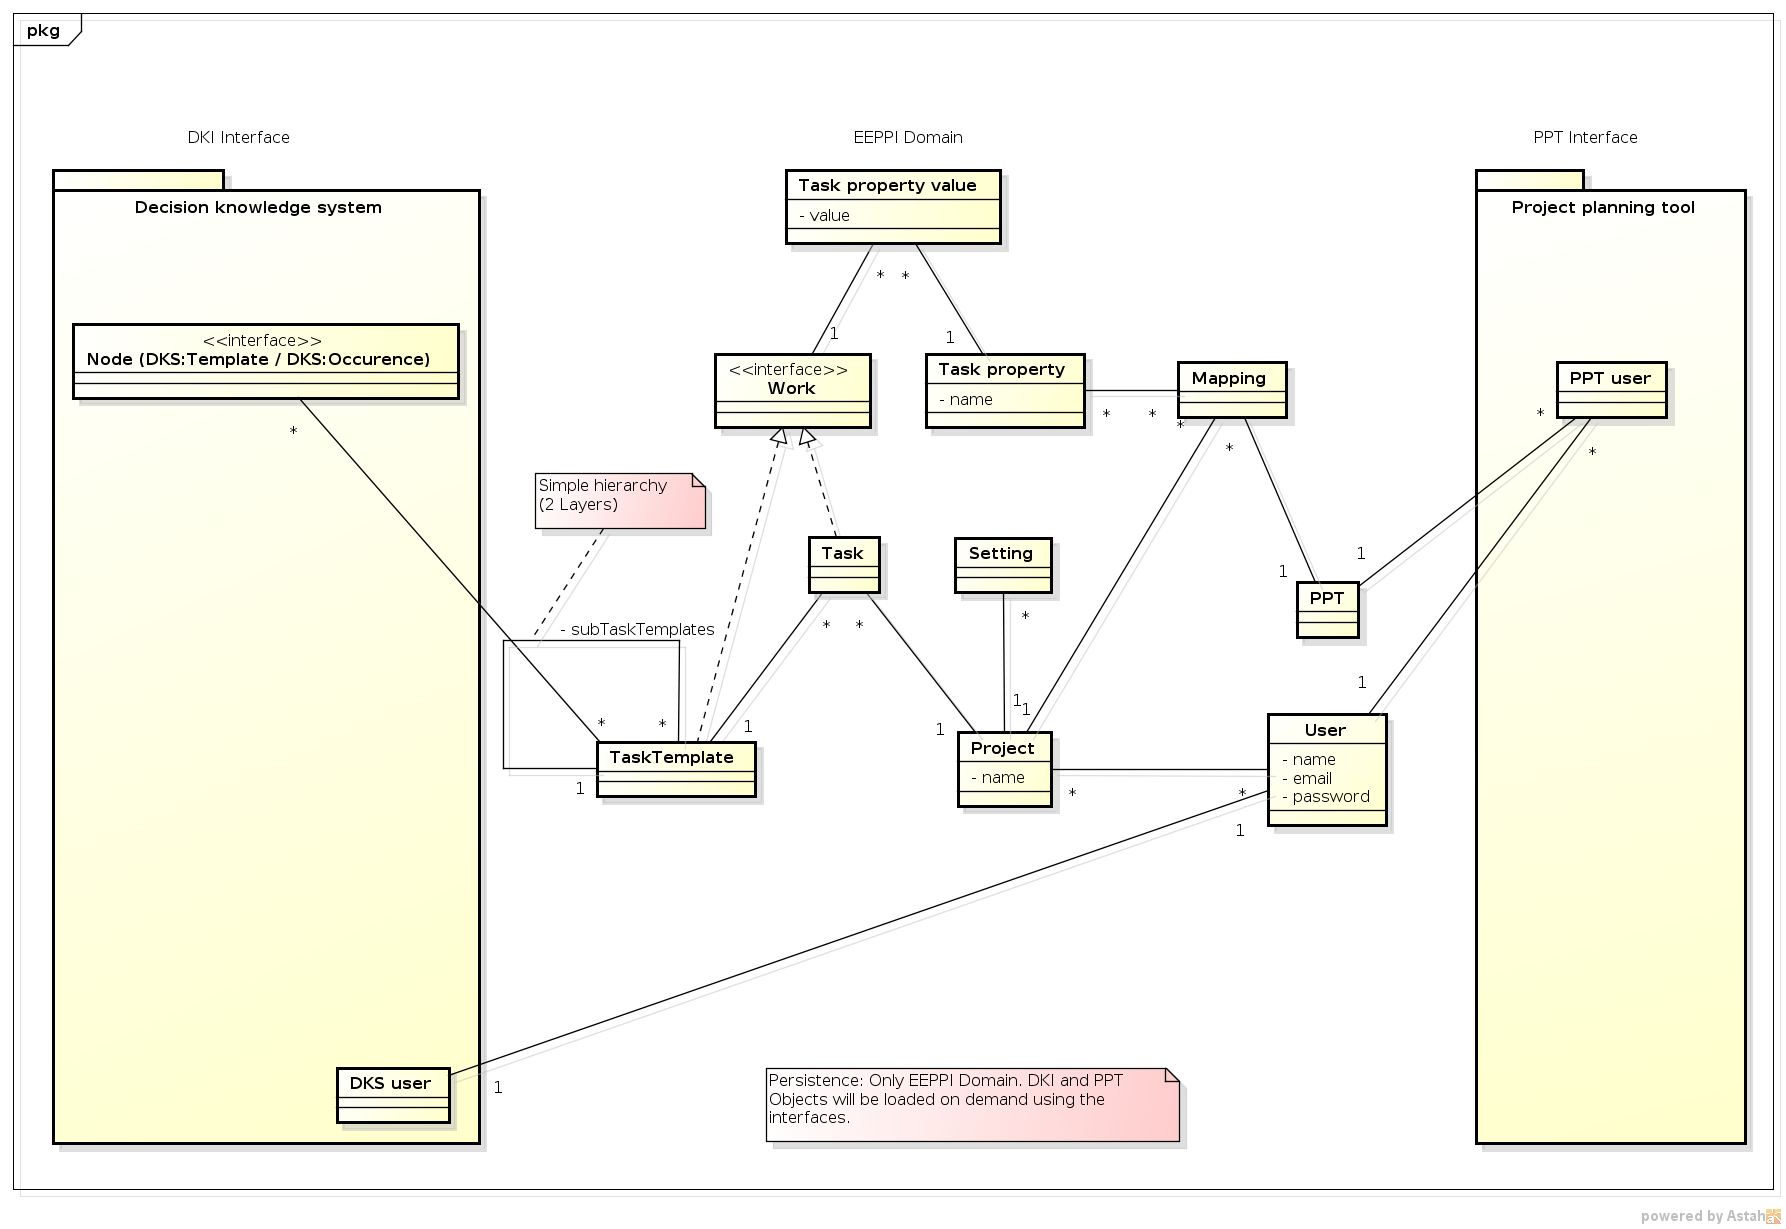
\includegraphics[width=0.9\linewidth]{architecture/media/img/domain.png}
					\centering
					\caption{Konzeptionelle \eeppi -Domäne}
					\label{fig:domain}
				\end{figure}				
			\end{landscape}
			
			\eeppi\ arbeitet mit den Objekten des \dks. Das ADRepo als Referenz-\dks\ ist wie folgt aufgebaut:
			\begin{figure}[H]
				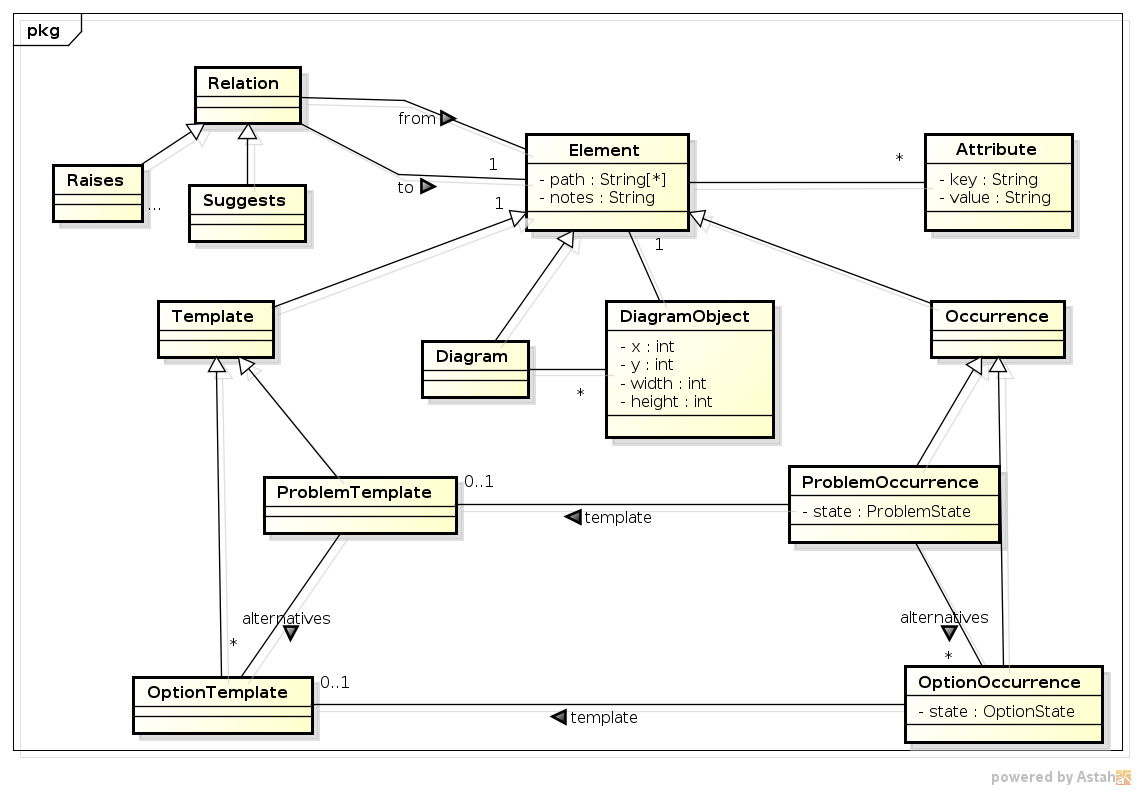
\includegraphics[width=\linewidth]{architecture/media/img/dksDomain.png}
				\centering
				\caption[ADRepo-Domäne\newline 
					\license{Eclipse Public License \url{https://www.eclipse.org/legal/epl-v10.html} Lukas Wegmann, IFS HSR \url{https://www.ifs.hsr.ch}}
				]{ADRepo-Domäne (Quelle: IFS HSR, Abbildungsverzeichnis)}
				\label{fig:dksDomain}
			\end{figure}
			
			Dabei werden die Objekte wie folgt gemappt:
			\begin{description}
				\item[Element] Node
				\item[ProblemTemplate] Problem
				\item[ProblemOccurrence] Decision
				\item[OptionTemplate] Alternative
				\item[OptionOccurrence] Option
			\end{description}
			
			
		\subsection{Metamapping}
			\label{subsec:metamapping}		
		
			Metamapping bezeichnet das Konzept, 
			wie die Domäne des \dks s (DKS) und die \eeppi -Domäne verknüpft werden sollen.
			Übergreifend gesehen geht es dabei um nichts Geringeres als die Verbindung von Entscheidungsmanagement und Projektmanagement.			
		
			\begin{figure}[H]
				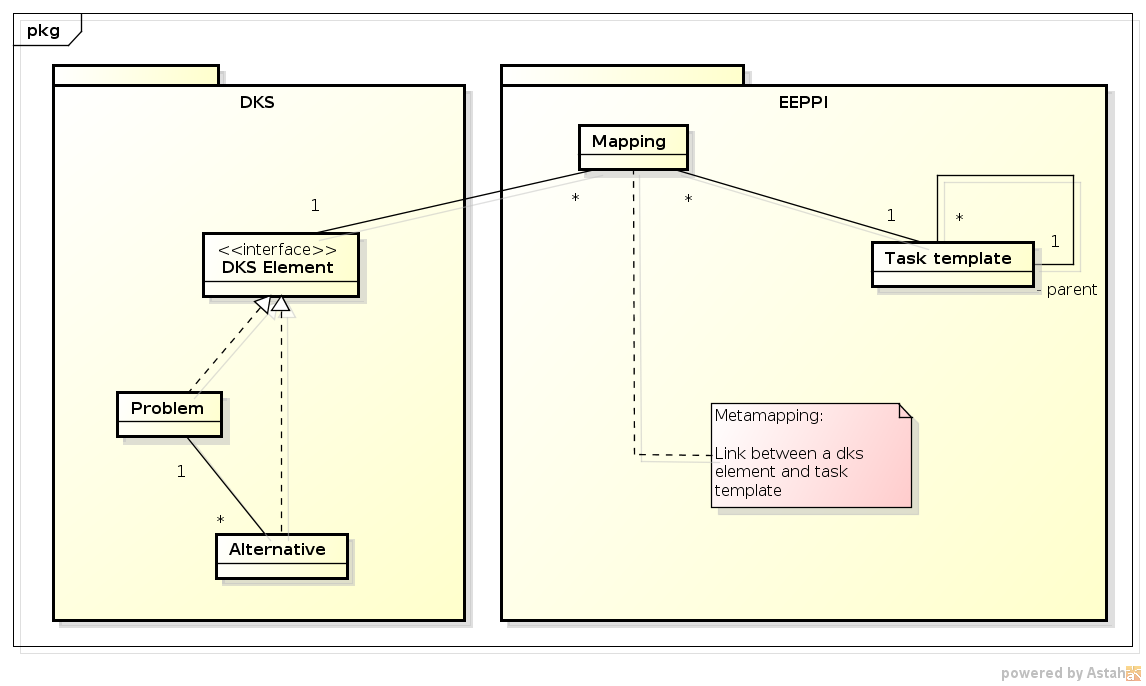
\includegraphics[width=\linewidth]{architecture/media/img/metaMapping.png}
				\centering
				\caption{Metamapping}
				\label{fig:metamapping}
			\end{figure}		
			
			Dazu wird die \dks -Domäne von \eeppi\ abstrahiert und mit Task\-tem\-plates verknüpft.
			Jedes Mapping steht für eine Verknüpfung eines \ttpl s mit einem Problem oder einer Alternative.
			
			Beim Erzeugen von konkreten Tasks müssen zu jedem Mapping alle Occurrences (siehe ADRepo-Domäne Abbildung \ref{fig:dksDomain}) gefunden werden.
			Anschliessend können zusammen mit den Daten des \ttpl s und dessen Eigenschaften (siehe \eeppi -Domäne Abschnitt \ref{fig:domain}) Tasks erzeugt werden.
			
			
		\subsection{Implementationsdomäne}
			Die konzeptionelle Domäne von \eeppi\ berücksichtig auch mögliche Erweiterungsaspekte.
			Die Implementationsdomäne bricht aus der konzeptionellen die Teilmenge heraus, die effektiv umgesetzt wird und konkretisiert diese.
			
			\begin{landscape}
				\begin{figure}[H]
					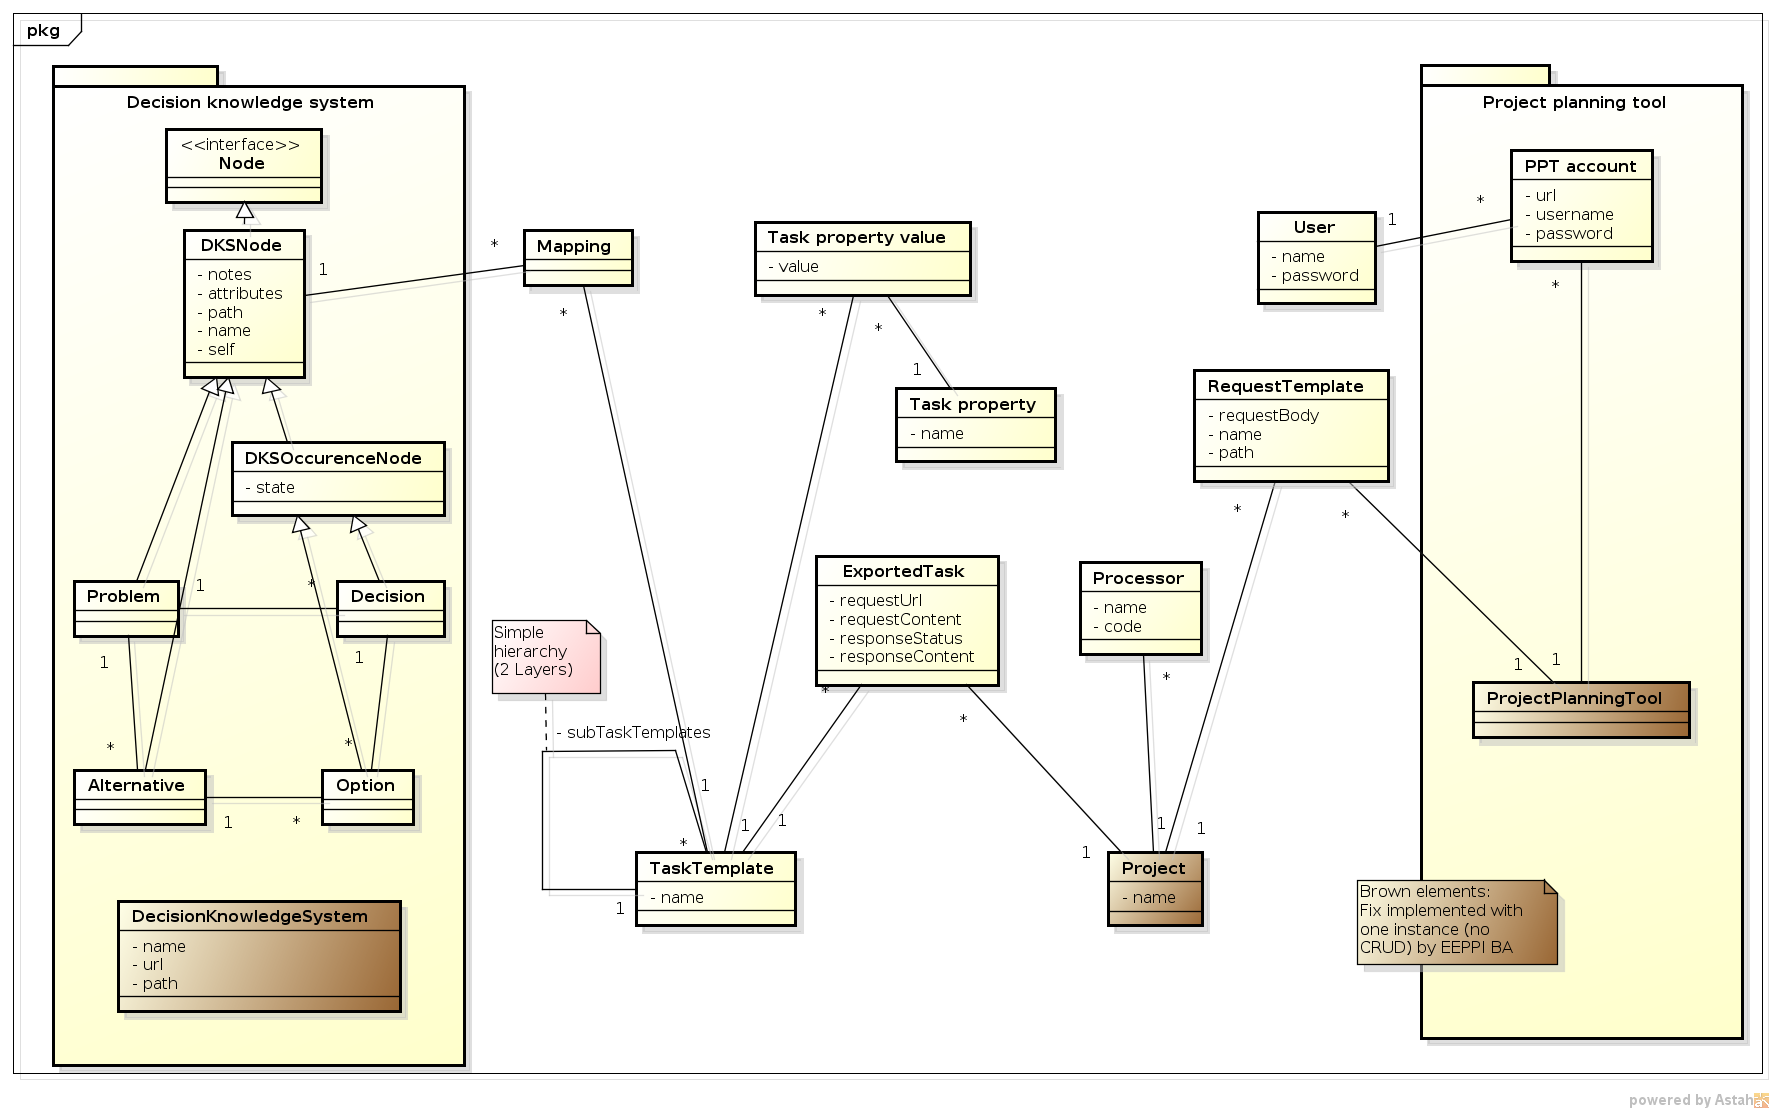
\includegraphics[width=0.9\linewidth]{architecture/media/img/implementationDomain.png}
					\centering
					\caption{\eeppi -Implementationsdomäne}
					\label{fig:implementationDomain}
				\end{figure}				
			\end{landscape}	
			
			Ebenfalls enthält die Implementationsdomäne die Abstraktion der DKS Objekte.
			Sie zeigt auch das gegenüber der konzeptionellen Domäne einfacher gehaltene Benutzer- und Projekt-Konzept.
			
			
		\subsection{Umbenennen und Löschen von Domänenobjekten}
			Um Probleme mit referenzierten Domänenobjekten zu vermeiden,
			darf es Benutzern nur möglich sein, \ttpl s umzubenennen,
			nicht jedoch zu löschen.			

			Das Löschen von referenzierten \ttpl s würde dazu führen, 
			das ein Teil der Export-Historie verloren gienge und Mappings kein zugeordnetes \ttpl\ mehr besitzen würden.
			 Dies wiederum würde zu fehlerhaften Exports, bzw. leeren Exports führen.
			 Aus diesem Grund ist das Löschen von referenzierten \ttpl s keine Option, höchstend das Löschen von noch nicht referenzierten.			
			
			Könnten Benutzer \ttpl s löschen, so müsste geprüft werden, 
			ob diese referenziert werden. Sobald der Benutzer jedes \ttpl einmal exportiert hätte, könnte er ebenfalls keines mehr löschen.
			Die Möglichkeit zum Löschen ist entsprechend sowieso nur in einem neu aufgesetzten System gegeben.
			
			Das konsequente Umsetzen der "<Umbenennen statt Löschen">-Strategie ermöglich Benutzern, 
			falsch angelegte \ttpl s weiterzuverwenden, vermeidet jedoch, 
			dass sich die Applikation unterschiedlich verhält für bereits referenziert und noch nicht referenzierte \ttpl s.
			
			Das Gleiche gilt auch für Task Properties.
			Dies dürfen auf keinen Fall vom Benutzer entfernt werden 
			und dürfen entsprechend nur umbenannt werden.
			
		
		\subsection{\ttpl s Strukturierung}
			Es gibt verschiedene Möglichkeiten, 
			Benutzer eine Strukturierung von \ttpl s anzubieten.
			\ttpl s können selbst in eine Struktur gebracht werden
			oder durch externe Strukturen geordnet werden.
		
			\begin{figure}[H]
				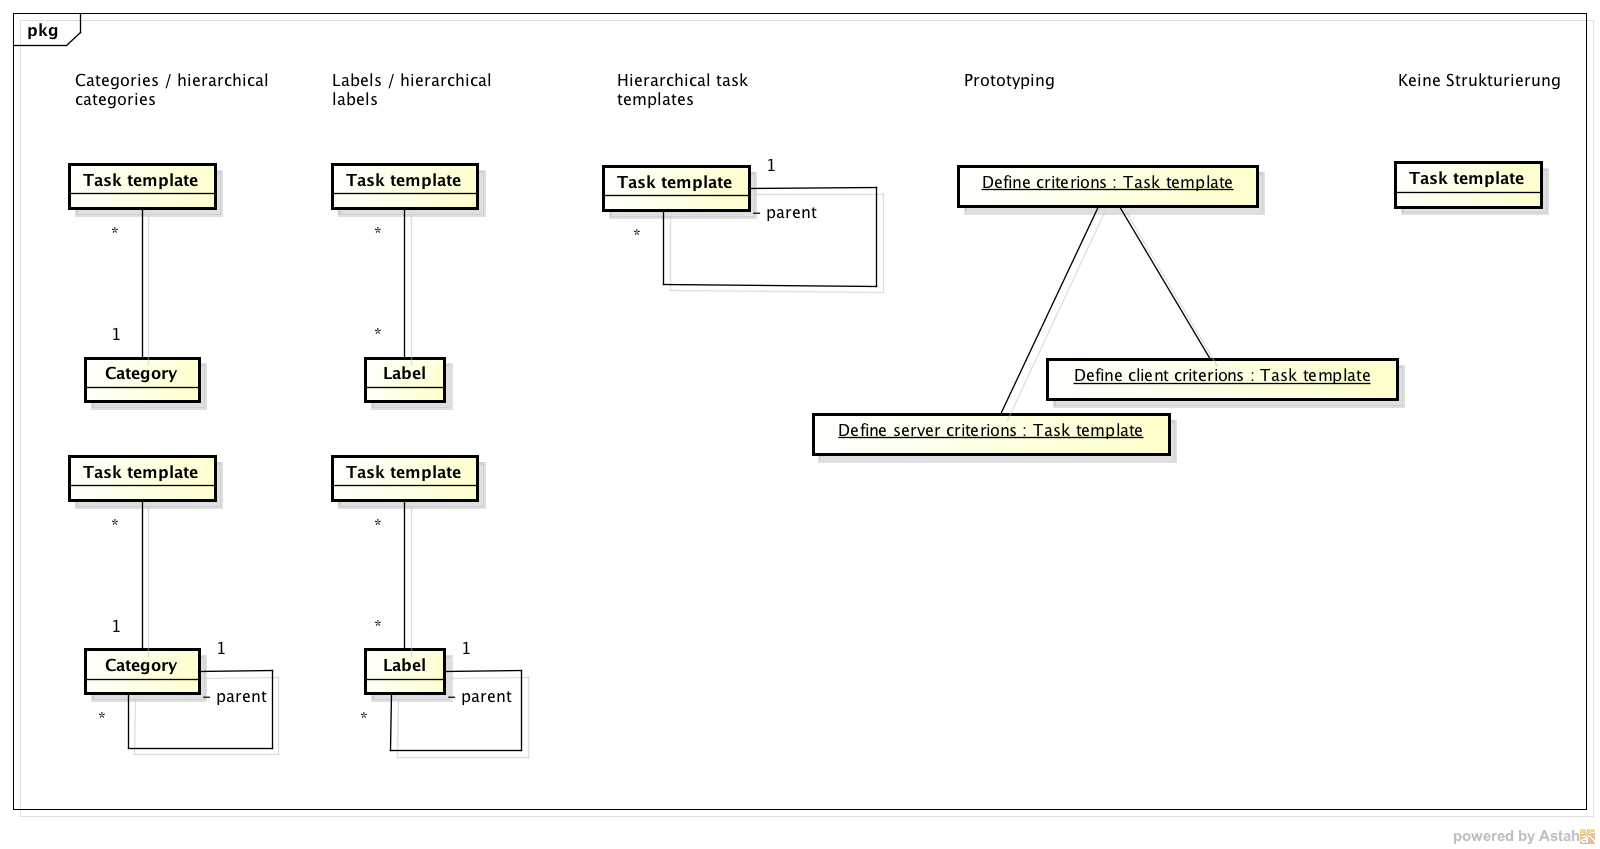
\includegraphics[width=\textwidth]{architecture/media/img/taskTemplateStructure.png}
				\centering
				\caption{Strukturierungsmöglichkeiten von Tasks}
				\label{fig:taskTemplateStructure}
			\end{figure}
			
		\decision{
			\decisionHeader{DOM-TT-STRUC}{\ttpl s Strukturierung}{Architecture}{Domain}
		}{
			\decisionContent{Keine Strukturierung, allenfalls auf Wunsch des Vertreters der Anforderungsgruppe nicht hierarchische Kategorien, Smart Filters}
			{Welches Konzept soll zur Strukturierung von \ttpl s eingesetzt werden?}
			{\ppt\ s unterstützen überhaupt hierarchische Tasks, ansonsten sind entsprechende Strukturierungsmöglichkeiten wenig sinnvoll}{Benutzer sollen einfach und schnell erstellte \ttpl s wieder finden.}
			{
				\begin{description}
					\item[Keine Strukturierung] \
						\begin{description}
							\item[Vorteile] Einfach zu implementieren, einfach verständlich für den Benutzer
							\item[Nachteile] Bei vielen \ttpl s unübersichtlich, führt zu doppelten \ttpl s,
							da existierende nicht gefunden werden. 
						\end{description}
						
					\item[Labels/Hierarchische Labels] \
						Versehen der Elemente mit einem oder mehreren Labels. Benutzer können nach Labels suchen oder Filtern, um Vorlagen anzuzeigen.	
						\begin{description}
							\item[Vorteile] Einfach verständlich für den Benutzer
							\item[Nachteile] Benutzer könnten zu faul sein, 
								Labels anzulegen und zuzuordnen da es aufwändiger ist, als Kategorisieren
						\end{description}
					
					\item[Direkte Hierarchisierung der \ttpl s] \
						Elemente werden direkt mit Elternelementen verknüpft und bilden einen hierarchischen Baum.	
						\begin{description}
							\item[Vorteile] Einfach zu implementieren
							\item[Nachteile] Schwer verständlich für den Benutzer,
								 da die Hierarchisierung unter Umständen nicht mit dem Workflow zusammenpasst
						\end{description}
					
					\item[Prototyping statt Strukturierung] \
						Elemente erben Funktionalität von einander, statt strukturiert zu werden.
						\begin{description}
							\item[Vorteile] Verringert die Anzahl \ttpl s massiv, 
								da Eigenschaften vererbt werden können
							\item[Nachteile] Schwieriger umzusetzen, schwieriger zu verstehen für Benutzer
						\end{description}					
				\end{description}
			}
			{
				Keine Strukturierung hat für die Entwicklung sowie für den Benutzer Vorteile.
				So gibt es zu diesem Punkt kaum Entwicklungsaufwand 
				und der Benutzer findet trotzdem dank Suchfunktionen die gesuchten \ttpl s.
				Ausserdem muss er keine Zeit aufwenden um die \ttpl s zu strukturieren.

				Falls Vertreter der Anforderungsgruppe jedoch eine weitergehende Strukturierung wünschen, 
				empfehlen wir nicht-hierarchische Kategorien sowie Smart Filters.
				Kategorien erlauben eine Strukturierung auf einfache Weise. 

				Smart Filter sind eine Ergänzung zu den beiden Optionen und ermöglichen das schnelle Finden anhand von Eigenschaften,
				ohne dass diese der Benutzer erfassen muss.
			}
			{keine}
			{Mögliche zukünftige Erweiterung durch Strukturierungsmöglichkeiten muss bei der Implementation berücksichtigt werden}
			{keine}
		}
		
		
		\subsection{Verknüpfungen von \ttpl s und Entscheidungs-Vorlagen}
			Wissensproduzenten können \ttpl s mit Problems (Entscheidungs-Vorlagen) verknüpfen.
			Dabei kann und soll ein \ttpl\ verschiedenen Problems zugeordnet werden können.
			Ebenso können Problems natürlich mehrere \ttpl s zugeordnet erhalten.
			
			\subsubsection{Arten der Zuordnung}
				\ttpl s können mit Problems auf zwei Arten verknüpft werden:
				\begin{enumerate}
					\item Sie können dann fällig werden, wenn eine Entscheidung getroffen wurde (operativer Task).
					\item Ein \ttpl\ dient dazu, Entscheidungen zu treffen (Entscheidungstask).
				\end{enumerate}
				Auf die \ttpl s selbst hat dies keinen Einfluss, sie sind unabhängig davon. 
				Ob es sich um einen operativen Task oder einen Entscheidungstask handelt, hängt nur davon ab,
				ob das \ttpl\ mit einem Problem oder einer Alternative einer Entscheidung verknüpft ist.
				
				Sollte eine Unterscheidung dennoch einmal notwendig sein, 
				so kann dies mittels Processors umgesetzt werden (Siehe Abschnitt \ref{subsec:transmissionWorkflow}), da die Daten des \dks s Typeninformationen enthalten.
				

			\subsection{Übertragung von Tasks in ein \ppt}
				Aus \ttpl s werden beim Übertrag in ein \ppt\ Tasks generiert.
								
				\ttpl s sind generische Vorlagen, die ständig weiterentwickelt werden sollen durch den Projektplaner.
				Aus diesem Grund wäre es unpraktisch, wenn ein Benutzer zur Änderung einer Vorlage für jedes Mapping alle \ttpl s anpassen müsste.
				Die Anzahl \ttpl s, die der Benutzer aktualisieren müsste, würde mit der Anzahl Mappings wachsen und schnell eine unüberblickbare Menge erreichen.
				
				Darum werden \ttpl s mit Mappings verknüpft (referenziert) und nicht kopiert zum Zeitpunkt des Mappings. 
				Eine Kopie würde für jedes Mapping eine neue Instanz des Tasktemplates erzeugen, 
				hätte jedoch zum Vorteil, das für bereits exportierte Tasks weiterhin die vor der Änderung verwendete Version des \ttpl\ erhalten bliebe.
				
				Passt der Benutzer nun ein \ttpl\ an und exportiert anschliessend Tasks, 
				so wird für alle gemappten Problems das aktuelle \ttpl\ verwendet,
				weil deren Verknüpfungen nur auf ein einziges \ttpl\ zeigen.
				
				\begin{figure}[H]
					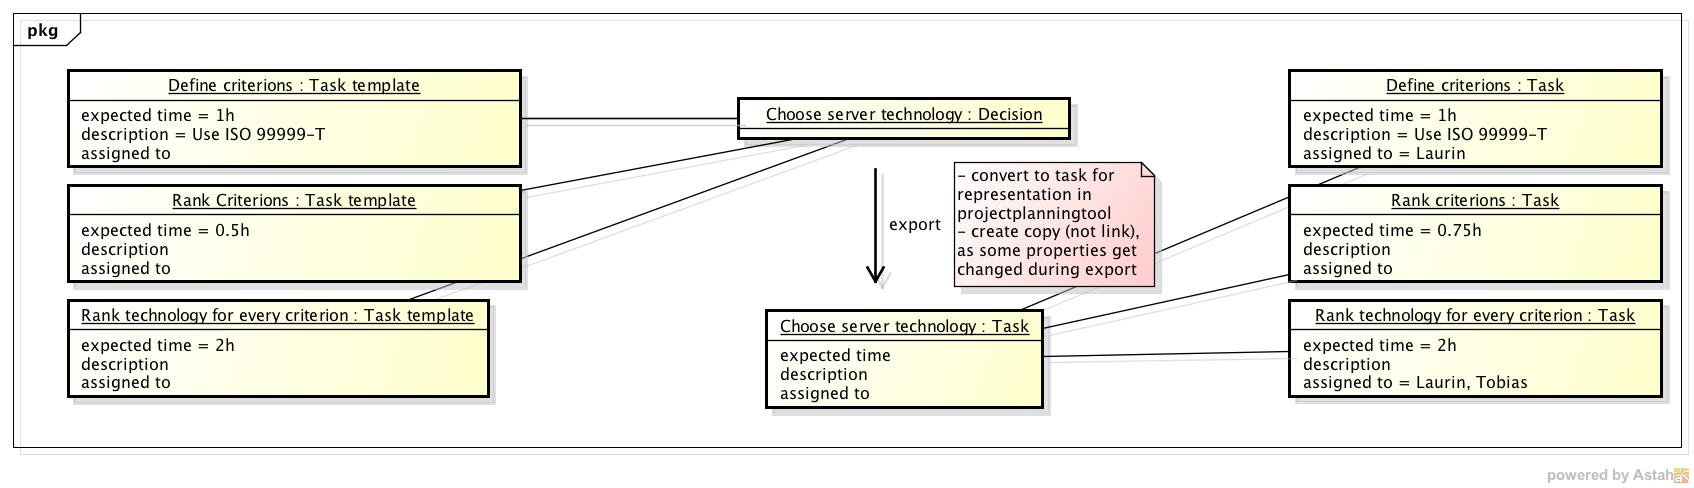
\includegraphics[width=\textwidth]{architecture/media/img/decisionTaskRelation.png}
					\centering
					\caption{Übertragen von Entscheidungen und \ttpl s}
					\label{fig:DecisionTaskRelation}
				\end{figure}
				
				Beim Übertragen werden aus \ttpl s (konkrete) Tasks.
				Mit Alternatives verknüpfte Tasks werden entsprechend zu Sub-Tasks.
				
				Benutzer wollen bei der Übertragung ins \ppt\ die vom \ttpl\ vorgegebenen Werte möglicherweise anpassen, wie zum Beispiel den erwarteten Aufwand für den Task.
				Daher ist es sinnvoll, die Eigenschaften der \ttpl s in die (konkreten) Tasks zu kopieren, anstatt sie lediglich zu verknüpfen.
				Gleiches gilt für Eigenschaften von Entscheidungen. Würde jemand im \dks\ diese verändern oder löschen,
				so würde dies die History zerstören.
			
		
		\subsection{Transmission-Workflow}
			\label{subsec:transmissionWorkflow}		
		
			Aus \ttpl s erzeugte Tasks müssen zur Übertragung in ein \ppt\
			umgewandelt werden, sodass die angesprochene API die Daten auch versteht. 
			Dazu werden "<Processors"> eingesetzt.
			
			\subsubsection{Processors}
			Processors stellen kleine Funktionalitäten dar, die Daten umwandeln.
			Beispiele für Processors sind:
			
			\begin{itemize}
				\item "<Date processor">, der Kalenderdaten umwandelt
				\item "<Issue type processor">, der Issuetypen konvertiert
				\item "<User processor">, der Relationen zu Benutzern so umwandelt, dass das \ppt\ den User korrekt verknüpfen kann
				\item "<Conditional processor"> und "<Option processor">, die Bedingungen verarbeiten
			\end{itemize}
			
			Ebenfalls denkbar ist ein Processor, der Felder aggregieren kann und damit zum Beispiel nicht gemappte Felder in die Beschreibung überführen kann.
			
			\begin{figure}[H]
				\begin{lstlisting}
function(issueType) {
	if(issueType == 'Feature') {
		return 2;
	} else if(issueType == 'Bug') {
		return 3;
	} else {
		return 1; // 'Task'
	}
}
				\end{lstlisting}
				\centering
				\caption{Beispielprocessor für Issuetypes}
				\label{fig:exampleProcessorCodeForIssueTypes}
			\end{figure}
			
			\begin{figure}[H]
				\begin{lstlisting}
{
	"issue": {
		//...
		{
			//...
			"issue_type": $issueTypeProcessor:(taskTemplate.attributes.Type)$,
			//...
		}
	//...
}
				\end{lstlisting}
				\centering
				\caption{Processorverwendung in einem Requesttemplate}
				\label{fig:processorUsageInRequestTemplate}
			\end{figure}
			
			Das Codebeispiel zeigt einen Processor, der textuelle Issuetypes auf ID's des \ppt\ abbildet.
			Der im Template verwendete "<issueTypeProcessor">-Aufruf wird mit dem Rückgabewert der Processorfunktion ersetzt, sodass für den Wert "<Feature"> für das \ttpl -Attribut "<Type"> 
			die folgende Zeile resultiert:
			
			\begin{figure}[H]
				\begin{lstlisting}
"issue_type": 2,
				\end{lstlisting}
				\centering
				\caption{Requesttemplate nach dem Ausführen des Processors}
				\label{fig:requestTemplateAfterProcessorCall}
			\end{figure}
			
			Weitere Beispiele für Processors und eine Anleitung um selbst welche in ein Requesttemplate zu integrieren,
			finden sich im Abschnitt \ref{chapter:userManual}, eine Auflistung über die zur Verfügung stehenden Inputdaten für Processors im Abschnitt \ref{sec:ExampleProcessorData} im Anhang.
			
			
			\subsubsection{Variables}
			Variables können auf Daten von \ttpl und Decision zugreifen,
			diese aber nicht verändern.
			
			\begin{figure}[H]
				\begin{lstlisting}
//...
"estimated_time": ${taskTemplate.attributes.Duration},
//...

				\end{lstlisting}
				\centering
				\caption{Verwendung von Variables in einem Requesttemplate}
				\label{fig:usageOfVariablesInRequestTemplates}
			\end{figure}
			
			
			\subsubsection{Verarbeitung und Übertragung}			
			Die folgende Grafik zeigt den kompletten Ablauf beim Verarbeiten ung Übertragen von Tasks.
			
			\begin{figure}[H]
				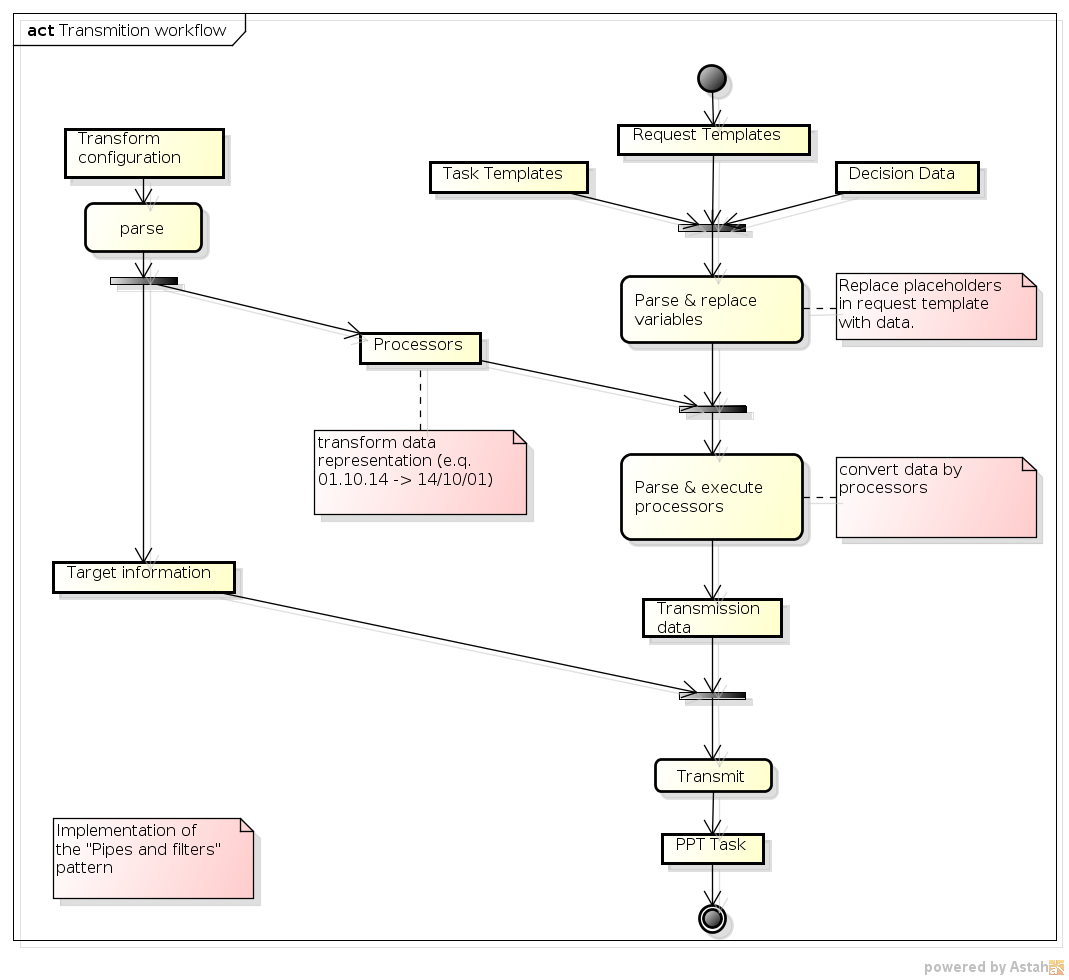
\includegraphics[width=\textwidth]{architecture/media/img/transmissionWorkflow.png}
				\centering
				\caption{Übertragen von Tasks}
				\label{fig:transmissionWorkflow}
			\end{figure}
			
			Dem Transmissionworkflow liegt das "<Pipes and filters">-Pattern zugrunde
			 \cite{hope_enterprise_2003}, welches eine Verarbeitungs- und Filterkette definiert.
			 Die Processors stellen dabei die "<Filters"> dar.
			
			Der komplette Transmittion-Workflow soll auf dem Client durchgeführt werden und nicht auf dem Server. 
			Die Wahl der Servertechnologie schränkt die Möglichkeiten für dynamische Processors ein, während die Client Technologie dies ermöglicht.
			
			Im Laufe der Erarbeitung dieses Workflows wurde über die Verarbeitung nicht gemappter Eigenschaften diskutiert. 
			In einer frühen Projektphase wurde entschieden, diese in Listenform in die Beschreibung des Tasks überzuführen. 
			Die Entscheidung für ein sehr flexibles Mapping führte dazu, 
			dass dieser Anwendungsfall überflüssig wurde.
			Der Administrator kann selbst einen Processor definieren, der alle Felder in eine Liste überführt und zur Beschreibung des Task hinzufügt.
			
			Die Vorteile dieser Lösung liegen auf der Hand: Die Entscheidung darüber, 
			wie mit nicht gemappten Feldern umzugehen ist, kann der Administrator treffen
			und die Entwicklung unsererseits vereinfacht sich.
			
			
			\subsubsection{Secondary Processors und Variables}
			Processors und Variables werden vor dem Übertragen der Information ausgeführt.
			Informationen, die erst zur Zeit der Übertragung bekannt sind, können somit nicht durch Processors und Variables abgerufen werden.
			
			Dafür sind sogenannte "<Secondary Processors"> notwendig, 
			die direkt vor dem Übertragen ausgeführt werden.
			Diese können Informationen über hierarchisch höher stehende Tasks (Elterntasks)
			abrufen und für das Template aufbereiten. So ist beispielsweise eine Verknüpfung zwischen Eltern- und Sub-Tasks realisierbar.
			
			Secondary Processors und Variables benutzen eine ähnliche Syntax\footnote{Anstelle des \$ am Anfang beginnen sie mit \$!} wie gewöhnliche Processors und Variables, 
			können jedoch nur auf die Daten der letzten Übertragung eines übergeordneten Tasks zugreifen.
			
			\begin{figure}[H]
				\begin{lstlisting}
{
	"issue": {
		//...
		{
			//...
			"parent_issue_id": $!{parentRequestData.issue.id}$,
			//...
		}
	//...
}
				\end{lstlisting}	
				\centering
				\caption{Beispiel für die Verwendung einer Secondary Variable zum Verknüpfen des Eltern-Tasks}
				\label{fig:secondaryProcessors}
			\end{figure}
			
		
		\subsection{Mapping Methode}
		\decision{
			\decisionHeader{DOM-TT-MM}{Mapping Methode}{Architecture}{Domain}
		}{
			\decisionContent{Konfiguration/Block in Form von Templates mit Platzhaltern}
			{Wie sollen Mappingkonfigurationen erstellt werden?}
			{Definiertes Konzept des Metamappings (Siehe Abschnitt \ref{subsec:metamapping})}
			{Von der Mapping Method hängt die Architektur des Mappings und die Schnittstellen der Processors und Filters ab.}
			{
				\begin{description}					
					\item[Hierarchische/Element basierte Konfiguration] \
					Das Mapping wird durch das Anlegen von verknüpften Elementen erzeugt.
					\begin{description}
						\item[Vorteile] Gegebene Validierung durch die Struktur, kein Parser notwendig
						\item[Nachteile] Aufwändiger umzusetzen, insbesondere das UI, weniger flexibel
					\end{description}
				\end{description}
			}
			{Eine Textblock/Template-basierte Konfiguration erhöht zwar die Fehlermöglichkeiten für den Administrator,
			ermöglicht diesem jedoch grössere Flexibilität und damit ein Abdecken einer grösseren Bandbreite an \ppt s.}
			{Der Administrator kann mit Templates und Platzhaltern umgehen oder es lernen}
			{Das Mapping benötigt kein eigenes Datenmodell in Form von verknüpften Objekten. 
			Es kann als einfache Text-Elemente an ein Projekt angeknüpft werden.}
			{Art der Speicherung in der Datenbank\footnote{In die Bachelorarbeit wurden nur die wichtigsten und grossen Entscheidungen eingefügt.}}
		}
		
		Der Ablauf für einen Administrator sieht entsprechend wie folgt aus:
		\begin{enumerate}
			\item \ppt\ definieren
			\item Taskeigenschaften erstellen
			\item Mapping Taskeigenschaften -> \ppt\ erstellen
		\end{enumerate}					
				
		
		\subsection{Kommunikation}
		\eeppi\ verwendet verschiedene Schnittstellen. Deren Verwendungen sind nachfolgend beschrieben.
			\subsubsection{Kommunikation zwischen \eeppi\ und dem \dks}
				Die Übertragung zwischen dem \dks\ und \eeppi\ basiert auf einer einer Ein-Weg-Kommunikation.
				\eeppi\ lädt die Daten, gibt jedoch keine Informationen zurück, ob dies erfolgreich war oder nicht.
				
				\eeppi\ schreibt auch keine Daten zurück ins \dks, wie beispielsweise Informationen über die Verwendung der Problems und Alternatives.
				Grund dafür ist die dazu notwendige Komplexität der Schnittstelle sowie die mangelnde Unterstützung seitens \dks.
				Auch würde diese Funktionalität den Rahmen der Arbeit sprengen, als mögliche Erweiterung von \eeppi\ ist sie jedoch denkbar.
				
			
			\subsubsection{Kommunikation zwischen \eeppi\ und dem \ppt}
				Die Übertragung der erzeugten Tasks ins \ppt\ basiert auf einer Zwei-Weg-Kommunikation.
				Zum einen werden die Tasks ans \ppt\ übertragen
				und zum anderen die Rückmeldung über die erfolgreiche Erzeugung der Tasks im \ppt\ wieder im \eeppi\ gespeichert.
				Ebenfalls zurückgeliefert werden minimale Informationen über den erstellten Task, 
				wie zum Beispiel die ID. 
				\eeppi\ verwendet diese Informationen, um dem Benutzer Secondary-Processors anzubieten, die zum Beispiel Informationen über einen Parent Task in das Requesttemplate einweben.
				
				Der "<Transmission">-Workflow als Gesamtes ist jedoch ein One-Way-Procedure.
				Dies bedeutet, dass keine Daten aus dem \ppt\ zurück in \eeppi\ fliessen.
				Technisch zwar möglich, stellt eine Rückkopplung der Daten oder sogar eine Synchronisierung der Tasks eine grosse Herausforderung dar, 
				die den Rahmen der Arbeit sprengen würde.
				Als mögliche zukünftige Erweiterung ist dies jedoch denkbar und könnte eines
				der Schlüsselkriterien werden, warum Projektplaner \eeppi\ einsetzen wollen.